\documentclass[12pt,letterpaper,english,bibliography=totocnumbered, abstract=on]{scrartcl}

\usepackage{indentfirst}
\usepackage[titletoc]{appendix}
%\usepackage{fullpage}
%\usepackage{subfiles}
\usepackage[T1]{fontenc}
\usepackage[latin9]{inputenc}
\usepackage{color}
\usepackage{babel}
\usepackage{verbatim}
\usepackage[unicode=true,pdfusetitle,
bookmarks=true,bookmarksnumbered=false,bookmarksopen=false,
breaklinks=true,pdfborder={0 0 0},pdfborderstyle={},backref=false,colorlinks=true]
{hyperref}
\hypersetup{linkcolor=blue,citecolor=blue,urlcolor=blue}

\usepackage{booktabs}
\usepackage{multirow}
\usepackage{adjustbox}
\usepackage{threeparttable}
\usepackage[table]{xcolor}
\usepackage{csquotes}
\usepackage{soul} % for hiliting text: \hl

\usepackage[backend=biber, style=authoryear, maxbibnames=99, dashed=false]{biblatex}
\setlength\bibitemsep{2\itemsep}
%\addbibresource{mylibrary.bib}
\addbibresource{CRB.bib}

\usepackage{pdfpages}
\usepackage{float} % Allows use of H to place floats

\usepackage{pgfgantt}

\usepackage{framed}

% Prevent page breaks within paragraphs
% https://tex.stackexchange.com/questions/21983/how-to-avoid-page-breaks-inside-paragraphs
\widowpenalties 1 10000

\begin{document}

\titlehead{Grant Proposal: USDA Forest Service FY2020}

\title{Control of Little Fire Ant (LFA) and Coconut Rhinoceros Beetle (CRB) on Guam}

\author{Glenn Dulla PhD, Guam Department of Agriculture\\
	Aubrey Moore PhD, University of Guam}


\maketitle
%\footnote{\url{https://github.com/aubreymoore/2020-FS-CRB-biocontrol-project/blob/master/combined-proposal.pdf}}
\newpage
\tableofcontents

\pagebreak

\section{Combined Budget}

% Please add the following required packages to your document preamble:
% \usepackage{booktabs}
% \usepackage[table,xcdraw]{xcolor}
% If you use beamer only pass "xcolor=table" option, i.e. \documentclass[xcolor=table]{beamer}
\begin{table}[h]
	\centering
	\begin{tabular}{@{}lrrr@{}}
		\toprule
		\multicolumn{1}{c}{\textbf{Item}} & \multicolumn{1}{c}{\textbf{Cost(UOG)}} & \multicolumn{1}{c}{\textbf{Cost(GDOA)}} & \multicolumn{1}{c}{\textbf{Total}} \\ \midrule
		Personnel & \$66,200 & \$72,987 & \$139,187 \\
		Benefits & \$19,200 & \$0 & \$19,200 \\
		Travel & \$4,000 & \$0 & \$4,000 \\
		Supplies & \$0 & \$2,545 & \$2,545 \\ \midrule
		\multicolumn{1}{r}{\textbf{SUBTOTAL}} & \textbf{\$89,400} & \textbf{\$75,532} & \textbf{\$164,932} \\ \midrule
		Administrative fee & \$15,776 & \$13,329 & \$29,106 \\ \midrule
		\multicolumn{1}{r}{\textbf{TOTAL}} & \textbf{\$105,176} & \textbf{\$88,861} & \textbf{\$194,038} \\ \bottomrule
	\end{tabular}
\end{table}

\begin{description}
	
	\item [{Personnel (UOG)}] includes salary for an insect pathologist (Dr. James Grasela, 1 FTE, \$64,000) and benefits calculated at 30\% * salary. Also includes PI's salary compensation calculated at 0.02 FTE * \$110,000.

	\item [{Personnel (GDOA)}] Research Associate I, (fulltime, \$20.34/hour, 2080hrs)=\$42,307; 
	Research Assistant III (fulltime or 2x halftime, \$14.75/hour, 2080hrs)=\$30,680
	
	\item [{Travel (UOG)}] includes airfare and other relocation expenses for Dr. Grasela who resides in Missouri.
	
	\item [{Supplies (GDOA)}]  
	Fuel (7,488miles, work truck, 20MPG, \$4.50/gallon)=\$1,685; 
	Survey Supplies (peanut butter, chopsticks, fluorescent tape/flags, ziplock bags)=\$500; 
	Wrist Garmin GPS units (2x \$180)=\$360 	
	
	\item [{Administrative~fee (UOG and GDOA)}] equal to 15\% of the total grant award
	is charged by the Research Corporation of the University of Guam for
	services provided.
	
\end{description}


\pagebreak
\section{Little Fire Ant Management}
Please see next page.

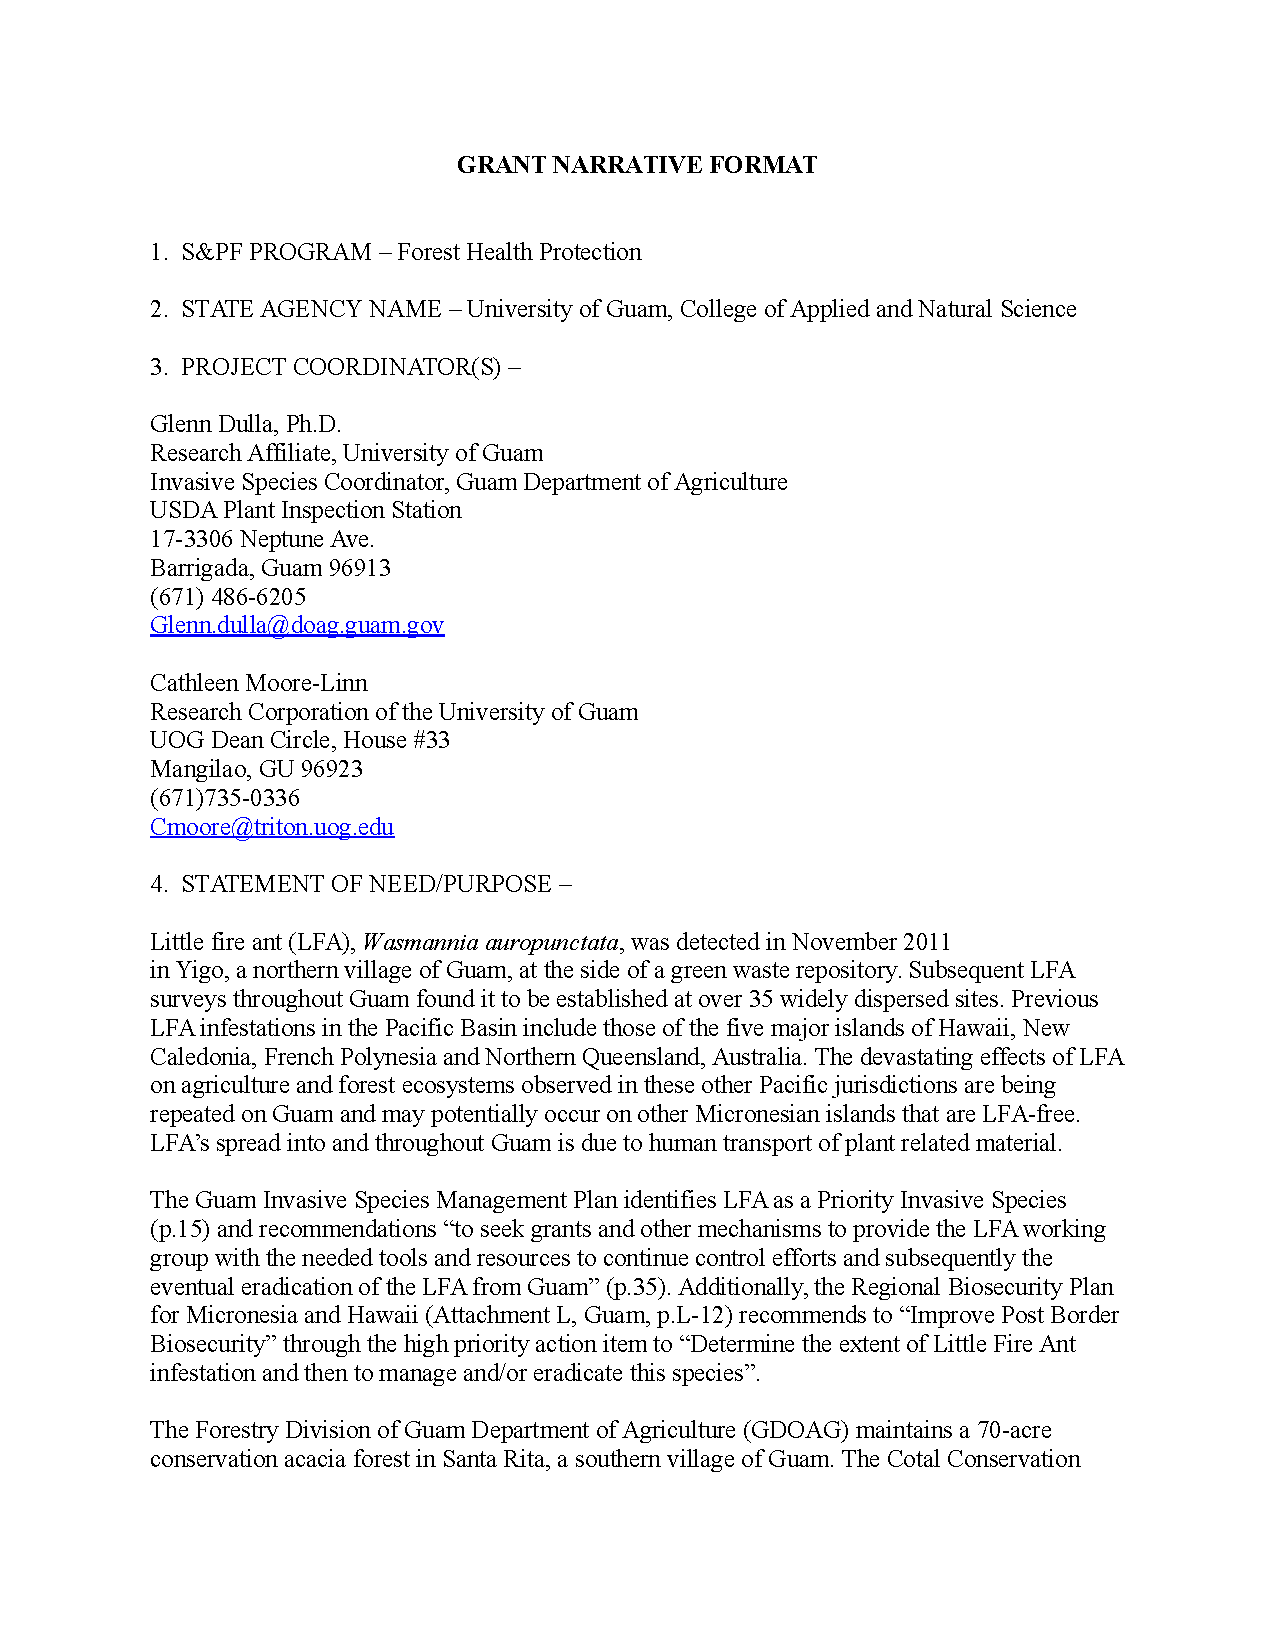
\includepdf[pages=-]{LFA-proposal.pdf}

\section{Coconut Rhinoceros Beetle Biological Control}
Please see next page.

If you want to use active hyperlinks in the attached document, please download from 
\tiny{\url{https://github.com/aubreymoore/2020-FS-CRB-biocontrol-project/blob/master/combined-proposal.pdf}}

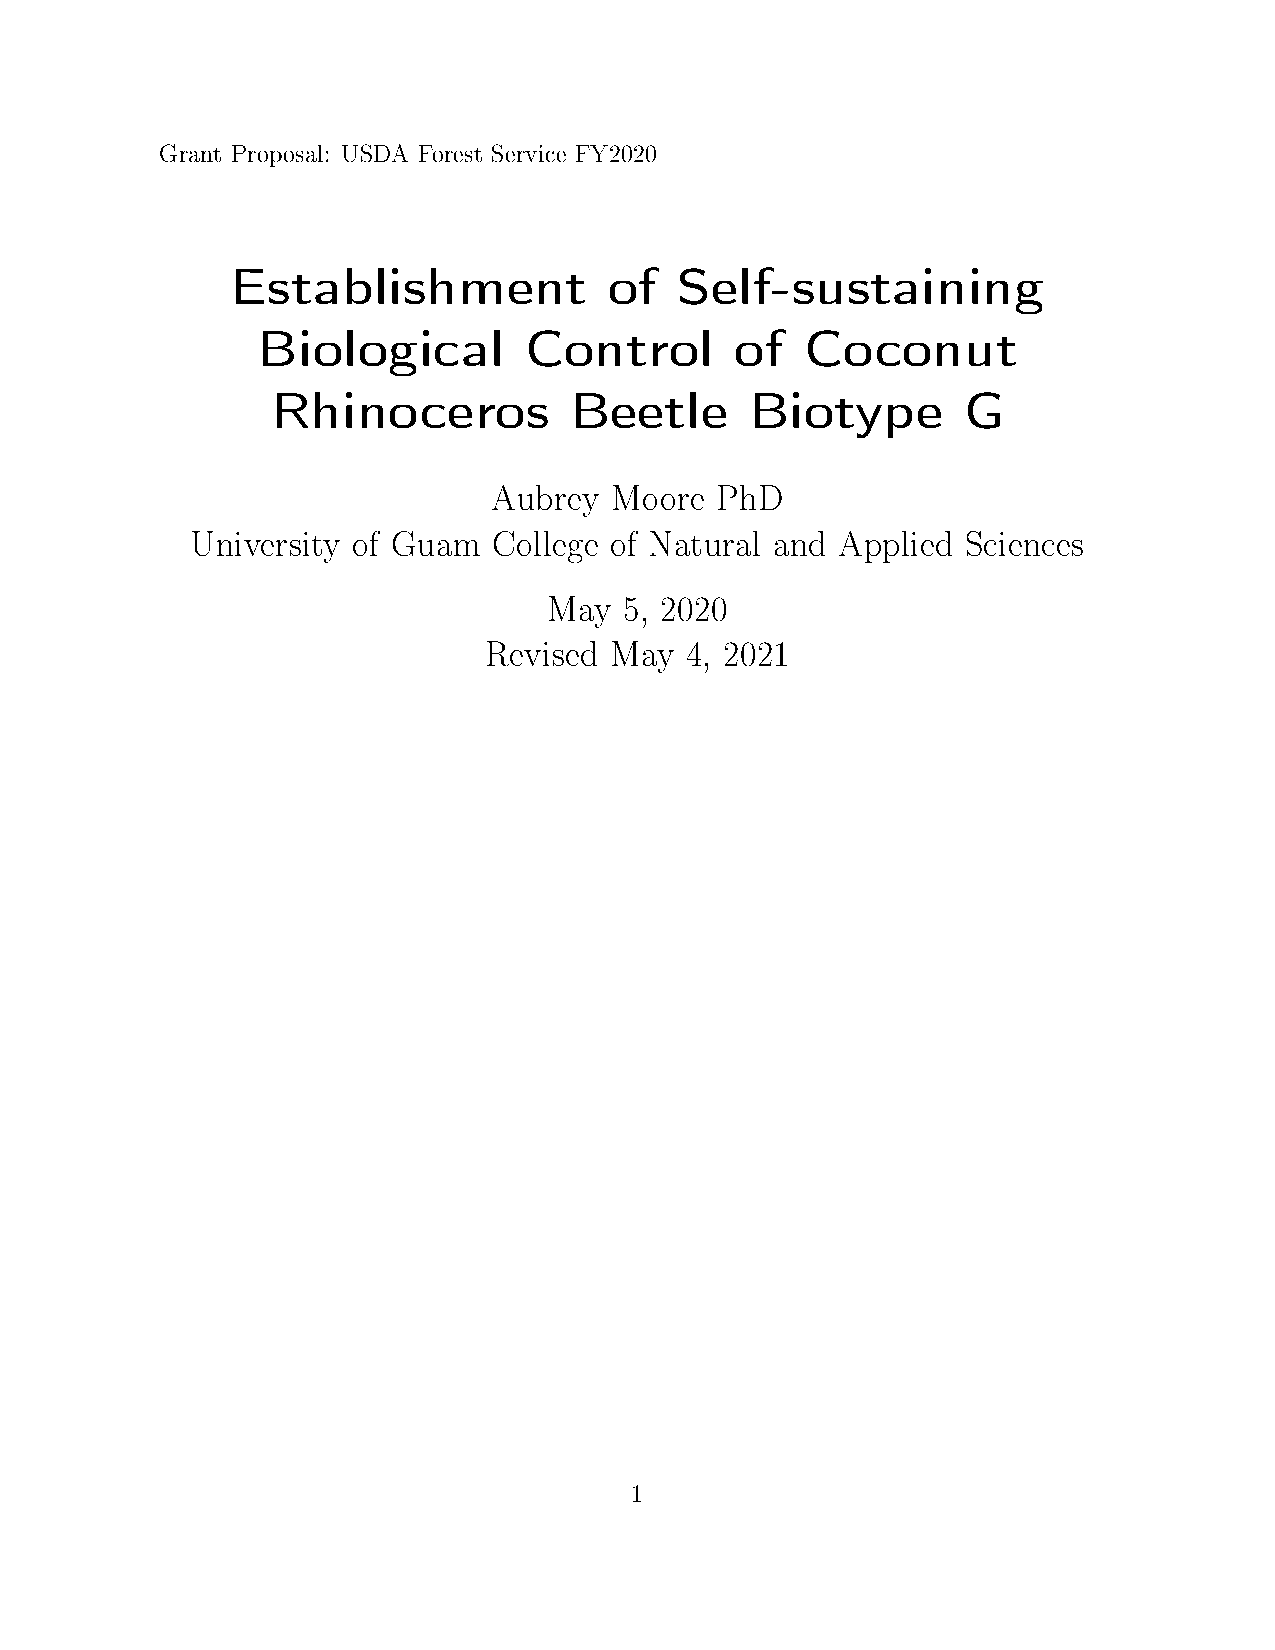
\includepdf[pages=-]{proposal.pdf}

\end{document}
